In this section we provide an overview of the SDN architecture and the types
of errors observed in production software-defined networks.

\subsection{SDN Architecture}

Modern SDN platforms are highly complex. We enumerate the characteristics of
these systems here.

In order to scale to large networks and achieve fault tolerance for the control
plane itself, SDN platforms distribute control state across cluster(s) of servers.
Onix~\cite{onix}, for example,
partitions a graph of the network state across either an eventually-consistent
DHT or a transactional database. Control applications can thus make their own
tradeoffs in choosing consistency models, degree of
fault tolerance, and other properties.

The modern SDN stack \colin{too general... it's really just Nicira's stack}
contains up to three layers: the lowest
layer is responsible for tracking switch state and pushing configuration
changes to the switches themselves; a virtualization layer
wraps the state of the network in a programmable abstraction; and a control
application written by network administrators 
expresses the network policy in terms of the virtualization layer abstraction.
A depiction of this architecture is shown in Figure \ref{fig:basicarch}.

The virtualization layer facilitates a concise specification of
intended network behavior. A common pattern is to represent an entire
datacenter network as a single logical switch. In this manner, operators
can specify routing, access control, and QoS policies by configuring a single forwarding
device; the platform then maps the configuration onto sequences 
of forwarding elements in the physical network.

Virtualization additionally facilitates multi-tenancy, and isolates control applications from the specifics
of the underlying network. Ideally, each application is reduced to a
state-less, side-effect free function:
\begin{align*}
f(view) \rightarrow configuration
\end{align*}

\begin{figure}[t]
    %\hspace{-10pt}
    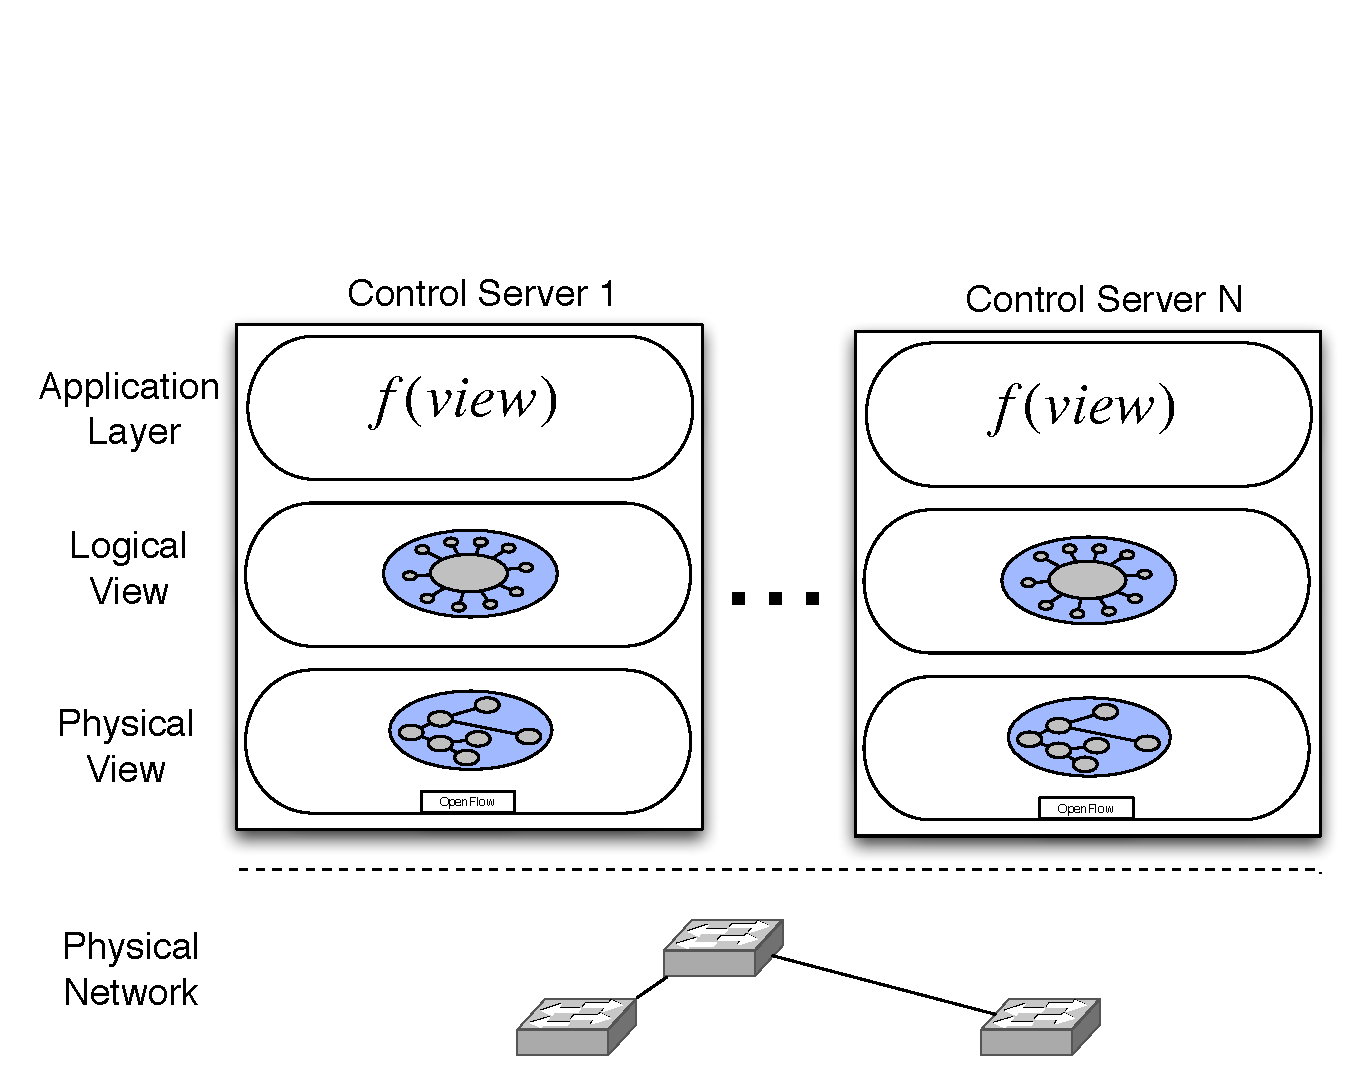
\includegraphics[width=3.25in]{../diagrams/architecture/SDN_Stack.pdf}
    \caption[]{\label{fig:basicarch} Depiction of the layered SDN stack.} 
\end{figure}

SDN controllers can be further categorized according to their flow
installation model: proactive or reactive.
Proactive controllers pre-compute forwarding tables for the entire network,
and only push down updates periodically to react to link failures, changes in
traffic mix, \etc. In contrast, reactive controllers forward all new flows to
control servers. After a control decision is made, a flow entry is installed
into the ingress switch, and the packet is forwarded along.
\colin{Mention that we focus on proactive? And that industry does too? :P}

\subsection{Platform Failure Modes}

Here we provide an overview of the platform's failure modes. Note that
we do not address failures in the highest (control application) and lowest
(dataplane forwarding tables) levels of abstraction. Previous work exists
for finding and troubleshooting faults in the application layer~\cite{nice}
and the forwarding plane~\cite{anteater}. We focus here on failure modes unaddressed
by this work.

As described in the previous section, modern SDN platforms differ from
`first-generation' controllers such as NOX~\cite{nox} in two dimensions. 
First, they extend vertically by providing a virtualization layer on top of
which control logic resides. Second, they extend horizontally by
distributing state across multiple control servers. Errors arise from both of
these architectural additions. Moreover, the sheer scale of production
SDN deployments amplifies the
frequency and severity of errors; consider that Microsoft reports 36M 
minor to fatal error events over one year across 8 datacenters,
which implies 8.5 error events per minute per
datacenter~\cite{Greenberg:2009:VSF:1592568.1592576}. Errors due to virtualization,
controller coordination, scale, and the confluence of these factors are the main
focus of our work.

\noindent{\bf Virtualization}. Virtualization errors often result from a mismapping between the logical
switch and the physical network topology. Consider that an entire datacenter
network (up to 10,000 switches) may be abstracted into a single logical switch. Especially in the
presence of hardware failures, the mapping between the logical switch and the
physical topology is highly complex. In a multi-tenant environment, the mapping is often
many-to-many~\cite{Casado:2010:VNF:1921151.1921162}; each tenant specifies
policies on their own logical switch, while the platform multiplexes each
slice over the same physical network. If the logical address
spaces are not disjoint, or a change in the physical network causes the paths
to temporarily overlap, breaches of tenant isolation or failure to properly
install configuration changes may occur,

\noindent{\bf Controller Coordination}. Coordination between controllers
entails the same classes of error
conditions that plague general distributed systems; inconsistent reads and
writes, race conditions over message arrivals, and unintended consequences of failover
logic are common. As an example, suppose a controller fails, and all the
switches under its purview are adopted by a new control server. If the new parent
fails to properly query the switches for their current state, or reads
stale control information from the data store, it may inadvertently install
conflicting flow entries in the network. Errors may also result as a
result of non-disjoint partitioning
schemes between controllers, or incorrect delegation of control for different
portions of the network. 
Moreover, consider that there may
be high churn in the network topology given VM migration or 
hardware failures. 

%All of these errors may manifest as dataplane forwarding problems, such as
%loops, blackholes, partitions, broadcast storms. Or breaches of isolation in
%multi-tenant environments. Or just failure to push routing or ACL or QoS
%policys to switches. Also Route flapping. Or (preventable) congestion.
